\section{Case Study 2: VAST Challenge 2014}
TimeSets was integrated into the visual analytics system SAVI~\cite{Xu2014} that won an award in the IEEE VAST Challenge 2014~\footnote{\url{http://www.vacommunity.org/VAST+Challenge+2014}}. The challenge is an annual contest with the goal of advancing visual analytics through competition. Commonly, participants are given a synthetic dataset and asked to identify suspicious activities within the dataset. The mini challenge that SAVI participated involves a fictitious company that has several employees have been missing. Participants had to collect and analyze streaming tweets in order to identify five interesting events before presenting hypotheses and evidence about the disappearance of the employees.

The SAVI interface consists of three panels (\autoref{fig:ts-savi}). At the bottom is a histogram showing the frequency of tweets over time. On the right hand side is the a collection of named entities identified from the entire dataset. Both components also act as filters. For example, when a user selects an interval of interest from the histogram, only tweets within that interval will be displayed in TimeSets, at the top-left corner of the interface. The user can select several entities to make TimeSets only show tweets mentioning at least one of these entities. TimeSets also uses the entities as \emph{sets}, allowing the user to observe the development of selected entities overtime.

\begin{figure}[!htb]
	\centering
	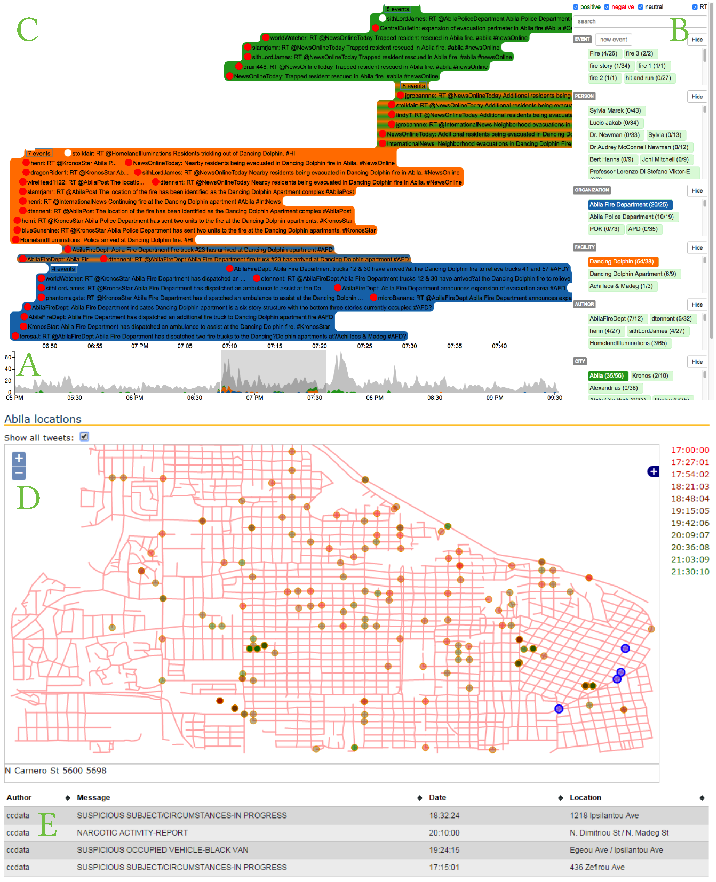
\includegraphics[width=\linewidth]{savi}
	\caption{SAVI interface. Bottom left: Histogram showing the frequency of tweets. Right: List of extracted named entities. Top left: TimeSets showing detailed tweets.}
	\label{fig:ts-savi}
\end{figure}

Besides showing tweets as raw data, TimeSets can also be used to construct and present interesting events. An event is described a sequence of related tweets organized in a chronological order. During the analysis, the analyst can create events and add tweets into one or many events. As a result, TimeSets allows the analyst to present an event together with its key elements. Also, by showing many events simultaneously, tweets that belong to multiple events can be identified and suggested further exploration to understand the connection among them.